\section{Problem 2} \label{sec:CST_implimented_Yagi}
\textit{ Using the CST microwave studio given at the course, design a Yagi-Uda antenna that has a gain of at least 6 dBi at 850 Mhz. Compare the results with the results from Matlab code }\\

We implemented the designed antenna from mm6 shown in \figref{fig:3_element_yagi-uda_geometry}. The simulation parameters for this simulation is shown in \tref{tab:antenna_param_CSTtime} and the design setup from CST is shown in \figref{}.

\ptable{| p{12cm} | p{6cm} |}{ %
Parameter 		&	Value 			\\ \hline
Reflector size 		        &	$0.482\lambda$	$\approx$ 170mm         \\ \hline
Dipole size 		        &	$0.5\lambda$	$\approx$ 176mm         \\ \hline
Director size 		        &	$0.424\lambda$	$\approx$ 150mm         \\ \hline
Reflector position (x axis) &	$0$	        							\\ \hline
Dipole position (x axis) 	&	$0.2\lambda$	$\approx$ 71mm	        \\ \hline
Director position (x axis) 	&	$0.2\lambda$	$\approx$ 71mm	        \\ \hline
Wire radius 		        &	$0.0085\lambda$	$\approx$ 3mm	        \\ \hline
Excitation lower freq 		        &	$\SI{350}{\mega\hertz}$	        \\ \hline
Excitation higher freq 		        &	$\SI{1.35}{\giga\hertz}$	    \\ \hline
}{Simulation and design parameters for CST in time domain}{tab:antenna_param_CSTtime} 
t 
\begin{figure}[!h]
  \centering
  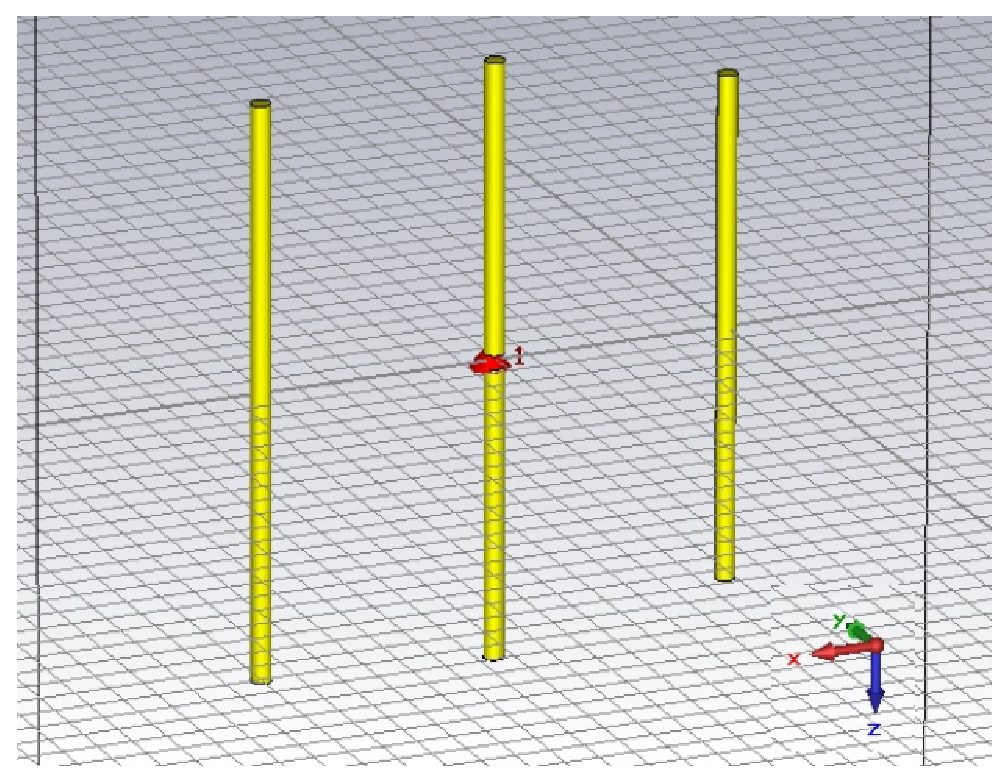
\includegraphics[width=10cm]{3_element_yagi_CST.eps}
  \caption{Figure showing the designed Yagi in CST. Note that the simulation box is much larger than shown in the figure.}
  \label{fig:3_element_yagi-uda_geometry}
\end{figure}

The designed Yagi antenna in CST is giving a gain patten as shown in \figref{fig:yagi_3D_pattern_CSTtime} when simulating in the time domain. The polar plot is shown in \figref{fig:yagi_pol_pattern_CSTtime} we can see that the three elements Yagi-Uda antenna presents a gain of 8.9dBi. In \figref{fig:yagi_cart_pattern_CSTtime} the Cartesian version is also presented.

\begin{figure}[!h]
  \centering
  \includegraphics[width=11cm]{yagi_3D_pattern_CSTtime.eps}
  \caption{Figure showing the 3D gain patten of the CST designed antenna in time domain.}
  \label{fig:yagi_3D_pattern_CSTtime}
\end{figure}

\begin{figure}[!h]
  \centering
  \includegraphics[width=11cm]{yagi_pol_pattern_CSTtime.eps}
  \caption{Figure showing the polar gain patten of the CST designed antenna in time domain.}
  \label{fig:yagi_pol_pattern_CSTtime}
\end{figure}

\begin{figure}[!h]
  \centering
  \includegraphics[width=11cm]{yagi_cart_pattern_CSTtime.eps}
  \caption{Figure showing the Cartesian gain patten for the CST designed antenna in time domain.}
  \label{fig:yagi_cart_pattern_CSTtime}
\end{figure}